\documentclass[12pt,a4paper]{book}

\usepackage{amsmath,amssymb,amsthm,amsfonts}
\usepackage{mathtools}
\usepackage{bm}

\usepackage{geometry}
\geometry{margin=2.5cm}

\usepackage{hyperref}
\usepackage{graphicx}

\usepackage{float}


\usepackage{setspace}
\linespread{1.7}

\usepackage[extrafootnotefeatures]{xepersian}
\settextfont[Scale=1.1]{XB Niloofar} % در صورت نیاز تغییر بده
\setlatintextfont{Times New Roman}
\setmathdigitfont{Yas}


\newtheorem{theorem}{قضیه} % ساختار ساده
\newtheorem{lemma}[theorem]{لم} % شماره‌گذاری وابسته به قضیه
\newtheorem{definition}{تعریف} % محیطی مستقل با شماره‌گذاری مجزا






\begin{document}
	
	%======================
	% Title Page
	%======================
	\begin{titlepage}
		\centering
		
		\vspace*{2cm}
		
		{\Huge \textbf{
{مقدمه‌ای بر تخمین جهت ورود سیگنال}
			}
		}\\[0.8cm]
		
		{
			\Large \lr{Introduction to Direction-of-Arrival Estimation}
		}
		
		\vspace{2cm}
		
		{\large نویسندگان:}\\[0.5cm]
		
		\lr{Zhizhang Chen\\
			Gopal Gokeda\\
			Yiqiang Yu}
		
		\vfill
		
		{\large مترجمان:}\\[0.5cm]
		محمد رضیئی فیجانی
		\\
	      محمد فخارزاده
		
		\vspace{1cm}
		
		{\large \today}
		
	\end{titlepage}
	
	%======================
	% Table of Contents
	%======================
	
	% !TeX root= ../DoABook.tex

\chapter*{پیشگفتار}

\textit{تخمین جهت ورود سیگنال}\LTRfootnote{Direction-of-Arrival} که اغلب به‌اختصار \lr{DOA} نیز گفته می‌شود (یا جهت‌یابی)، به‌طور اساسی به برآورد جهت ورود سیگنال‌ها می‌پردازد؛ سیگنال‌هایی که به‌صورت امواج الکترومغناطیسی یا آکوستیکی به یک حسگر یا آرایه آنتن برخورد می‌کنند. نیاز به تخمین جهت ورود سیگنال از کاربردهایی مانند جست‌وجو و نجات، اجرای قانون، سونار، لرزه‌شناسی و مکان‌یابی تماس‌های اضطراری $911$ در شبکه‌های بی‌سیم ناشی می‌شود.

در حوزه پردازش سیگنال آرایه‌ای، نظریه‌ها و روش‌های متعددی برای تخمین جهت ورود سیگنال توسعه یافته‌اند و ادبیات گسترده‌ای نیز پیرامون آن وجود دارد. با وجود این، در جریان پژوهش‌ها و پیاده‌سازی‌های عملی دریافتیم که منابع موجود بسیار پراکنده‌اند؛ به‌طوری‌که برای مبتدیان یا دانشجویانی که می‌خواهند در مدت‌زمانی کوتاه وارد این حوزه شوند، دسترسی به یک منبع یکپارچه دشوار است. به بیان دیگر، کتاب‌های مروری اندکی وجود دارند که اصول و تکنیک‌های پایه تخمین جهت ورود سیگنال را به‌صورت منظم و زیر یک سقف ارائه کنند.

این کتاب با هدف رفع این نیاز تألیف شده است و مروری یکپارچه بر الگوریتم‌های پایه تخمین جهت ورود سیگنال، تحلیل کارایی آن‌ها و مقایسه میان روش‌ها ارائه می‌دهد. به‌طور ویژه، توصیف‌های نظام‌مند، تحلیل کارایی و مقایسه انواع الگوریتم‌ها ارائه شده و در پایان تمرکز خاصی بر خانواده روش \lr{ESPRIT} قرار گرفته است؛ روشی که نام آن از \textit{تخمین پارامترهای سیگنال از طریق تکنیک‌های ناوردایی دورانی}\LTRfootnote{Estimation of Signal Parameters via Rotational Invariance Techniques} گرفته شده است.

این کتاب برای مبتدیانی نظیر دانشجویان تحصیلات تکمیلی، مهندسان یا نهادهای قانون‌گذار که باید در مدت کوتاهی با مبانی تخمین جهت ورود سیگنال آشنا شوند، مناسب است. همچنین برای متخصصانی که قصد مرور دوباره مبانی این حوزه را دارند سودمند خواهد بود. امید است که این کتاب اطلاعات نظری کافی درباره مبانی تخمین جهت ورود سیگنال در اختیار خواننده قرار دهد تا بتواند مفاهیم اولیه را درک کرده و در صورت تمایل به موضوعات پیشرفته‌تر وارد شود.







		
	\tableofcontents
	\newpage
	
	
	\twocolumnfootnotes
	% !TeX root = ../DoABook.tex
\chapter{مقدمه}
\label{chap:introduction}

کاربردهای فناوری‌های بی‌سیم در حوزه‌های گوناگونی گسترش یافته‌اند؛ از جمله پایش محیط‌زیست، شبکه‌های حسگر، امنیت عمومی و عملیات جست‌وجو و نجات. در پرتو این تحولات، سیاست‌ها و مقررات فناورانه متعددی برای پاسخ‌گویی به نیازهای مختلف تدوین شده‌اند. برای مثال، کمیسیون ارتباطات فدرال\LTRfootnote{Federal Communications Commission} در یک مقررات الزامی اعلام کرده است که دقت مکان‌یابی تماس‌های اضطراری بی‌سیم باید به $125$ متر برسد~\cite{1}. همچنین در عملیات جست‌وجو و نجات معمولاً تعیین مکان منابع بیکن الکترومغناطیسی ضروری است. همه این کاربردها را می‌توان از دلایل اصلی افزایش توجه اخیر به تعیین \textit{جهت ورود سیگنال‌های رادیویی}\LTRfootnote{Direction of Arrival} در سامانه‌های بی‌سیم دانست. در واقع، تخمین جهت ورود چندین سیگنال رادیویی که به یک آرایه از حسگرها برخورد می‌کنند، در بسیاری از کاربردهای دیگر نیز مورد نیاز است؛ از جمله رادار، سونار و لرزه‌شناسی. فناوری دیگری که در سال‌های اخیر توجه زیادی را به خود جلب کرده است، \textit{فناوری آنتن هوشمند}\LTRfootnote{Smart Antenna Technology} است~\cite{2,3}. در این فناوری معمولاً یک الگوریتم تخمین جهت ورود سیگنال به‌کار گرفته می‌شود تا سامانه‌هایی توسعه یابند که اطلاعات مکان‌یابی دقیقی برای خدمات بی‌سیم فراهم کنند~\cite{4}.

در چارچوب مباحث این کتاب، \textit{آنتن هوشمند} سامانه‌ای است که چندین المان آنتنی را با قابلیت پردازش سیگنال ترکیب می‌کند تا الگوی تابش و/یا دریافت خود را به‌صورت خودکار و متناسب با محیط سیگنالی سامانه بهینه کند. این فناوری به‌ویژه در ارتباطات سیار، با توجه به افزایش تعداد مشترکان و محدود بودن منابع، بسیار مفید واقع شده است. آنتن‌های هوشمند می‌توانند از طریق افزایش برد پوشش، محدوده سرویس‌دهی را گسترش دهند و همچنین ظرفیت سامانه را افزایش دهند~\cite{2,3}.

آنتن‌های هوشمند همچنین قادرند سیگنال‌ها را از نظر مکانی از یکدیگر جدا کنند؛ به‌گونه‌ای که مشترکان مختلف بتوانند از منابع طیفی یکسان استفاده کنند، مشروط بر آنکه در ایستگاه پایه از نظر مکانی قابل تفکیک باشند. این روش که \textit{دسترسی چندگانه با تقسیم فضایی}\LTRfootnote{Spatial Division Multiple Access} نامیده می‌شود، امکان می‌دهد چندین کاربر در یک سلول و روی یک فرکانس یا بازه زمانی یکسان فعالیت کنند؛ مشروط بر آنکه از تکنیک‌های \textit{پرتودهی تطبیقی}\LTRfootnote{Adaptive Beamforming} در آنتن‌های هوشمند استفاده شود. از آنجا که این رویکرد امکان پشتیبانی از کاربران بیشتری را در یک پهنای طیفی محدود فراهم می‌کند، در مقایسه با آنتن‌های متعارف می‌تواند به افزایش ظرفیت سامانه منجر شود.

فناوری آنتن هوشمند را می‌توان بر اساس راهبرد انتخابی در ارسال سیگنال به سه دسته اصلی تقسیم کرد:
\begin{itemize}
	\item روش \textit{لوب سوئیچی}\LTRfootnote{Switched Lobe (SL)}: این روش ساده‌ترین تکنیک بوده و تنها شامل یک تابع سوئیچینگ پایه میان پرتوهای از پیش تعریف‌شده یک آرایه است. هنگام دریافت یک سیگنال، تنظیمی که بهترین عملکرد را ــ معمولاً از نظر توان دریافتی ــ فراهم کند، برای عملکرد سامانه انتخاب می‌شود.
	
	\item روش \textit{آرایه فازی}\LTRfootnote{Phased Array (PA)}: این روش با استفاده از یک الگوریتم \textit{تخمین جهت ورود سیگنال} در سامانه، امکان ردیابی پیوسته منابع سیگنال را فراهم می‌کند؛ در نتیجه، ارسال از سوی آرایه می‌تواند به‌صورت هوشمند و بر اساس اطلاعات جهت ورود سیگنال کنترل شود. روش آرایه فازی را می‌توان تعمیمی از مفهوم لوب سوئیچی در نظر گرفت.
	
	\item روش \textit{آرایه تطبیقی}\LTRfootnote{Adaptive Array (AA)}: در این حالت، علاوه بر تعیین جهت ورود منبع مطلوب، یک الگوریتم تخمین جهت ورود برای تعیین جهت منابع تداخل ــ مانند سایر کاربران ــ نیز در سامانه به‌کار گرفته می‌شود. سپس الگوی پرتو به‌گونه‌ای تنظیم می‌شود که ضمن ایجاد صفر در جهت تداخل‌کننده‌ها، توان ارسالی در جهت منبع مطلوب بیشینه شود.
\end{itemize}
اهمیت تخمین \lr{DOA} در سامانه‌های آنتن هوشمند را می‌توان با بررسی ساختار این سامانه‌ها، همان‌گونه که در بخش بعدی تشریح می‌شود، به‌خوبی درک کرد.




\section{ساختار آنتن هوشمند}
\label{sec:smart-antenna-architecture}

ساختارهای متداول آنتن هوشمند برای یک ایستگاه پایه را می‌توان به بلوک‌های عملکردی زیر تقسیم کرد، همان‌گونه که در شکل‌های \ref{fig:1-1} و \ref{fig:1-2} نشان داده شده است:



\begin{figure}[h]
	\centering
	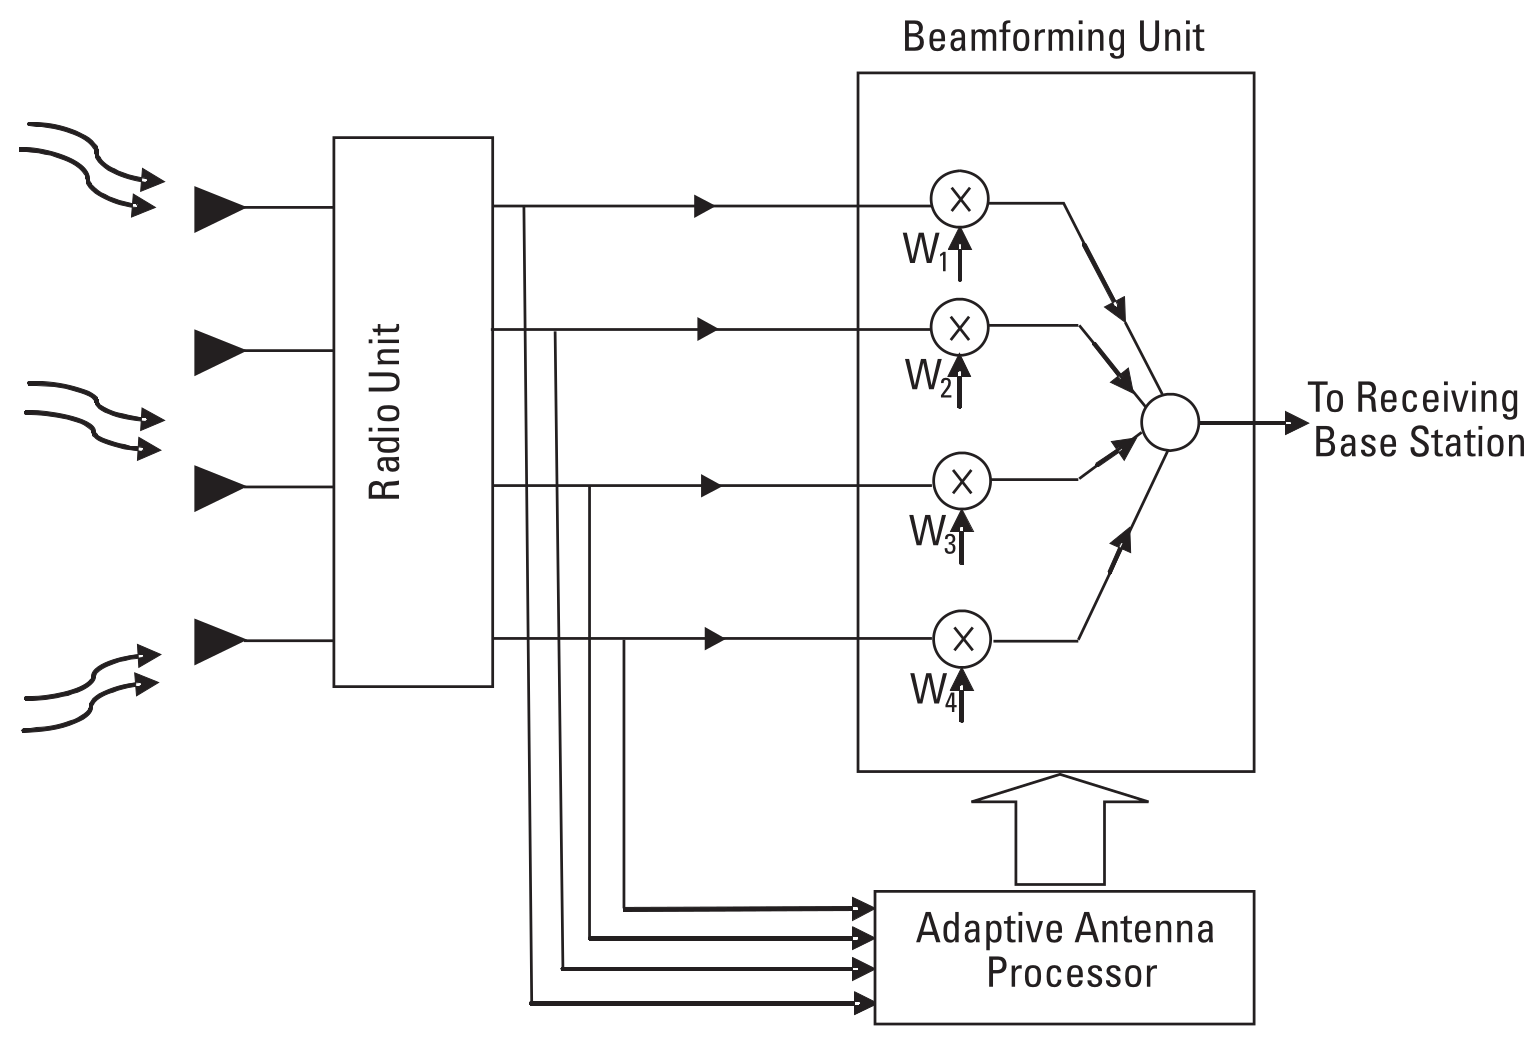
\includegraphics[width=0.7\linewidth]{chapters/figs/fig-1-1}
	\caption{گیرنده آنتن هوشمند}
	\label{fig:1-1}
\end{figure}

\begin{figure}[h]
	\centering
	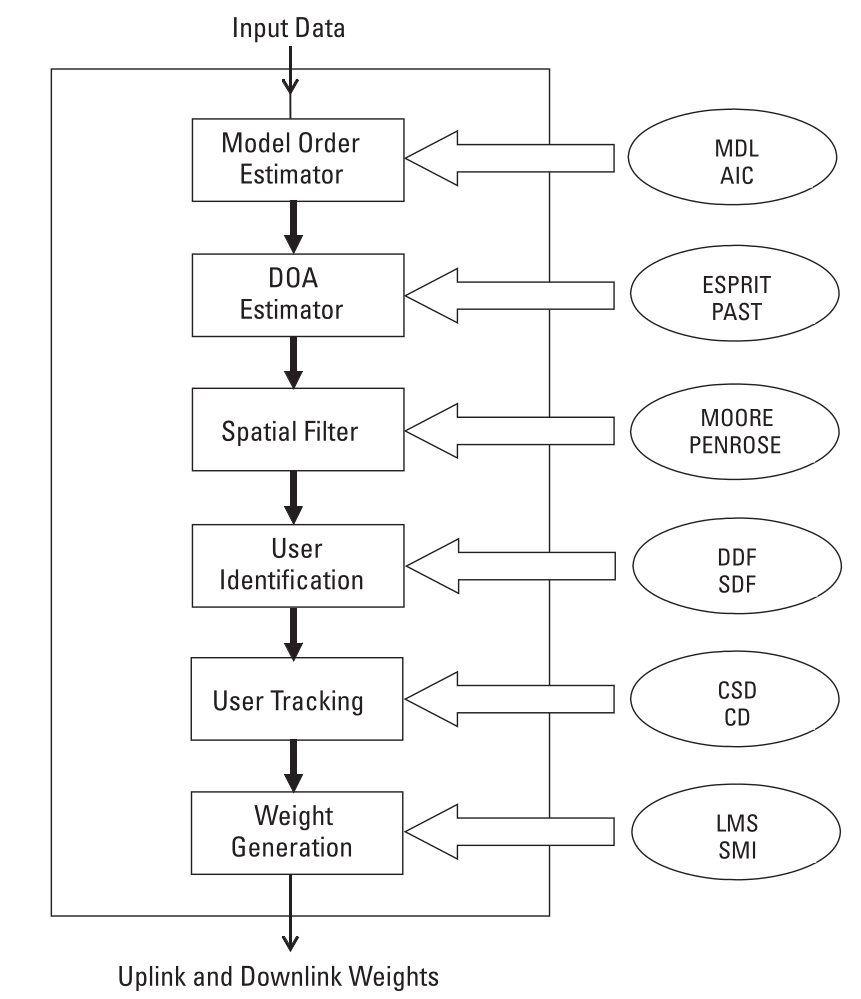
\includegraphics[width=0.7\linewidth]{chapters/figs/fig-1-2}
	\caption{پردازنده تطبیقی آنتن}
	\label{fig:1-2}
\end{figure}




\begin{itemize}
	
	\item \textbf{واحد رادیویی}\LTRfootnote{Radio Unit}:  
	این واحد عمدتاً شامل بخش‌های زیر است:  
	(1) آرایه‌های آنتنی که سیگنال‌های فرکانس رادیویی (\lr{RF}) را از محیط دریافت می‌کنند؛  
	(2) زنجیره‌های پایین‌تبدیل که حامل(های) سیگنال‌های \lr{RF} دریافتی توسط آرایه آنتنی را حذف می‌کنند؛  
	و (3) مبدل‌های آنالوگ به دیجیتال که سیگنال‌های بدون حامل را برای پردازش بیشتر به سیگنال‌های دیجیتال متناظر تبدیل می‌کنند.  
	
	آرایه‌های آنتنی می‌توانند یک‌بعدی، دوبعدی یا حتی سه‌بعدی باشند، بسته به اینکه بخواهیم به چه بعدی از فضا دسترسی داشته باشیم. الگوی تابش آرایه به نوع المان‌ها، موقعیت نسبی آن‌ها و تحریک هر المان (دامنه و فاز) بستگی دارد~\cite{5}.
	
	\item \textbf{واحد پرتودهی}\LTRfootnote{Beamforming Unit}:  
	واحد پرتودهی مسئول تشکیل و هدایت پرتو در جهت مطلوب است. در این بخش، وزن‌دهی به سیگنال‌های دریافتی (یا ارسالی) اعمال می‌شود. به‌طور کلی، سیگنال‌های داده $x_k$ با $k=0,\ldots,M-1$ که توسط یک آرایه با $M$ المان دریافت می‌شوند، مستقیماً در مجموعه‌ای از ضرایب وزن ضرب می‌شوند تا پرتویی در زاویه دلخواه تشکیل شود.  
	
	به بیان دیگر، با ضرب سیگنال‌های داده در مجموعه‌های مناسبی از وزن‌ها می‌توان مجموعه‌ای از پرتوها با زوایای نشانه‌روی دلخواه ایجاد کرد که نتیجه آن یک بیشینه سیگنال در خروجی پرتودهنده خواهد بود. از نظر ریاضی این رابطه به صورت زیر بیان می‌شود:
	\begin{equation}
		y(\theta_i) = \sum_{k=0}^{M-1} w_{k}^i \, x_k
		\label{eq:1-1}
	\end{equation}
	که در آن $y(\theta_i)$ خروجی پرتودهنده، $x_k$ نمونه داده از المان $k$ام آرایه و 
	
	$w_{k}^i$ وزن مربوط به تشکیل یک پرتو یا ایجاد صفر در زاویه $\theta_i$ است. توضیحات بیشتر درباره رابطه \eqref{eq:1-1} در فصل‌های \ref{chap:chapter2} و \ref{chap:chapter3} ارائه خواهد شد.
	
	با انتخاب مقادیر مناسب برای مجموعه وزن‌ها $w_k$ با $k=0,\ldots,M-1$ می‌توان عملیات هدایت پرتو، ایجاد صفر تطبیقی و شکل‌دهی پرتو را پیاده‌سازی کرد. این وزن‌ها که الگوی تابش را تعیین می‌کنند توسط واحد پردازنده تطبیقی آنتن تولید می‌شوند.
	
	\item \textbf{پردازنده تطبیقی آنتن}\LTRfootnote{Adaptive Antenna Processor}:  
	وظیفه این واحد تعیین وزن‌های مختلط برای واحد پرتودهی است. این وزن‌ها معمولاً بر اساس دو نوع معیار اصلی بهینه می‌شوند: بیشینه‌سازی سیگنال داده از منبع مطلوب (مانند روش‌های لوب سوئیچی یا آرایه فازی) یا بیشینه‌سازی نسبت سیگنال به تداخل (\lr{SIR}) از طریق سرکوب سیگنال منابع تداخل (در آرایه تطبیقی).
	
	از نظر تئوری، با $M$ المان آنتنی می‌توان $M-1$ منبع تداخل را حذف کرد، اما در عمل به دلیل انتشار چندمسیری، این تعداد معمولاً کمتر خواهد بود. روش محاسبه وزن‌ها بسته به نوع معیار بهینه‌سازی متفاوت است.
	
	در حالتی که از روش لوب سوئیچی استفاده شود، گیرنده تمام وزن‌های از پیش تعریف‌شده را آزمایش کرده و وزنی را انتخاب می‌کند که قوی‌ترین سیگنال داده دریافتی را ایجاد کند. اما اگر از روش آرایه فازی یا آرایه تطبیقی استفاده شود ــ که شامل هدایت بیشینه بهره به سمت قوی‌ترین مؤلفه سیگنال است ــ ابتدا جهت‌های ورود سیگنال‌ها (\lr{DOA}) تخمین زده می‌شوند و سپس وزن‌ها متناسب با\textit{ زاویه هدایت}\LTRfootnote{Steering angle} مطلوب محاسبه می‌شوند.
	
\end{itemize}
به‌طور کلی، همان‌طور که در شکل \ref{fig:1-2} نشان داده شده است، پردازشگر آنتن تطبیقی\LTRfootnote{Adaptive antenna processor} از چندین فرآیند محاسباتی تشکیل شده است:

\begin{itemize}
	\item \textbf{تخمین‌گر مرتبه مدل\LTRfootnote{Model order estimator}:} از روی داده‌های ورودی $\bm{x}_k$ برای $k = 0, \dots, M-1$ که توسط عناصر آنتن دریافت می‌شوند، تعداد جبهه‌های موج\LTRfootnote{Wavefronts} تابیده بر آرایه با استفاده از الگوریتم‌های تخمین مرتبه مدل، مانند \lr{AIC} یا \lr{MDL} تخمین زده می‌شود که در فصل \ref{chap:4} شرح داده خواهند شد. آگاهی از تعداد سیگنال‌های تابیده بر آرایه برای الگوریتم‌های تخمین جهت ورود\LTRfootnote{Direction of Arrival (DOA)} حیاتی است؛ از این رو، این الگوریتم‌ها پیش از الگوریتم‌های تخمین \lr{DOA} اجرا می‌شوند.
	
	\item \textbf{تخمین‌گر \lr{DOA}:} این بخش، مرحله حیاتی پردازشگر آنتن تطبیقی را تشکیل می‌دهد که در آن از الگوریتم‌هایی مانند \lr{MUSIC} یا \lr{ESPRIT} برای تخمین جهت ورود تمامی سیگنال‌های تابیده بر آرایه استفاده می‌شود. این مرحله، \lr{DOA}های تمامی سیگنال‌های مرتبط با منابع کاربر و سایر منابع تداخل را ارائه می‌دهد. برای سرعت بخشیدن به فرآیند، به‌جای تخمین فضای سیگنال در هر مرحله، از الگوریتم‌های رهگیری زیرفضا\LTRfootnote{Subspace tracking} مانند \lr{dPAST} و \lr{PAST} (رهگیری زیرفضا با تقریب تصویر\LTRfootnote{Projection Approximation Subspace Tracking}) برای رهگیری بازگشتی زیرفضای سیگنال استفاده می‌شود. معمولاً زیرفضای سیگنال به‌کندی با زمان تغییر می‌کند؛ بنابراین رهگیری این تغییرات نسبت به انجام تخمین کامل زیرفضا کارآمدتر است. سپس می‌توان \lr{DOA}ها را با سرعت بیشتری از این زیرفضاها تخمین زد. توصیفات دقیق این الگوریتم‌های \lr{DOA} در فصل‌های \ref{chap:3}، \ref{chap:4} و \ref{chap:5} ارائه شده است.
	
	\item \textbf{فیلتر مکانی\LTRfootnote{Spatial filter}:} پس از به‌دست آمدن \lr{DOA}های تمامی سیگنال‌های تابیده بر آرایه، سیگنال‌ها با بازسازی برای هر یک از \lr{DOA}های تخمین‌زده‌شده، فیلتر می‌شوند. تخمین سیگنال‌ها از روی \lr{DOA}های تخمین‌زده‌شده معمولاً بازسازی سیگنال\LTRfootnote{Signal reconstruction} یا کپی سیگنال\LTRfootnote{Signal copy} نامیده می‌شود. با در اختیار داشتن \lr{DOA}ها، بردارهای هدایت\LTRfootnote{Steering vectors} متناظر $\bm{a}$ و در نهایت ماتریس هدایت\LTRfootnote{Steering matrix} تخمینی $\bm{A}$ تشکیل می‌شوند. سپس سیگنال از رابطه زیر بازسازی می‌شود:
	\begin{equation}
		\bm{S} = \bm{W}\bm{X}
		\label{eq:1-1}
	\end{equation}
	که در آن $\bm{S}$ ماتریس سیگنال‌های تابیده است که از سیگنال‌های آلوده به نویز (یا سیگنال‌های داده) دریافت شده توسط آرایه $\bm{X}$ استخراج شده است، و ماتریس وزن‌دهی $\bm{W}$ به‌عنوان شبه‌معکوس مور-پنروز\LTRfootnote{Moore-Penrose pseudo inverse} ماتریس هدایت آرایه تخمینی $\bm{A}$ انتخاب می‌شود. جزئیات بیشتر در فصل \ref{chap:3} ارائه شده است.
	
	\item \textbf{شناسایی کاربر\LTRfootnote{User identification}:} زمانی که سیگنال‌ها با توجه به \lr{DOA}های متمایزشان از هم جدا شدند، کاربر موردنظر متناظر با این \lr{DOA}ها باید شناسایی شود. با مقایسه میان‌آیندهای\LTRfootnote{Mid-ambles} دریافت شده (توالی‌های آموزشی\LTRfootnote{Training sequences}) با میان‌آیند کاربر موردنظر، تعداد خطاهای بیتی در توالی آموزشی قابل محاسبه است. زمانی که تعداد خطاهای بیتی از یک آستانه کمتر باشد، یک جبهه موجِ تفکیک‌شده‌ی مکانی و در نتیجه \lr{DOA} متناظر با آن به یک کاربر نسبت داده می‌شود. به این ترتیب، نه تنها یک مسیر واحد، بلکه تمام مسیرهای متعلق به کاربر موردنظر شناسایی می‌شوند. سپس \lr{DOA} مربوط به مسیر کاربر با قوی‌ترین توان لحظه‌ای آشکارسازی می‌شود. به‌عنوان آشکارساز توالی آموزشی، تخمین‌گرهای توالی استاندارد مانند بازخورد تصمیم تأخیری\LTRfootnote{Delayed Decision Feedback (DDF)} و بازخورد تصمیم نرم\LTRfootnote{Soft Decision Feedback (SDF)} به کار می‌روند \cite{6}.
	
	\item \textbf{رهگیری کاربر\LTRfootnote{User tracking}:} یک تخمین‌گر تطبیقی با واکنش سریع برای رهگیری تغییرات پارامترهای سیگنال مورد نیاز است. رهگیر نه تنها از مختل شدن شکل‌دهی پرتو\LTRfootnote{Beamforming} توسط تخمین‌های پرت جلوگیری می‌کند، بلکه مانع از تغییرات بیش از حد تخمین‌های \lr{DOA} بین دو بسته‌ی سیگنال متوالی می‌شود. این امر منطقی است، زیرا یک کاربر متحرک در زمان واقعی طی یک فریم مشاهده، جابجایی زیادی ندارد؛ بنابراین تغییرات \lr{DOA} تدریجی است. رویکرد رهگیری کاربر بر پایه فرمول‌بندی بازگشتی برای رهگیری \lr{DOA}ها استوار است که در آن، تغییرات کوچک در تفاضل تخمین‌های ماتریس همبستگی، منجر به تغییرات کوچک در تفاضل ماتریس‌های هدایت می‌شود که \lr{DOA}ها از طریق آن‌ها استخراج می‌شوند. یکی از مشکلاتی که این الگوریتم‌ها ایجاد می‌کنند، مسئله تناظر داده‌ها\LTRfootnote{Data association} است؛ یعنی نسبت دادن تخمین‌های \lr{DOA} در لحظه زمانی قبلی به لحظه زمانی فعلی. برای غلبه بر این مشکل، الگوریتم‌هایی مانند تندترین نزول مقید\LTRfootnote{Constrained Steepest Descent (CSD)}، تندترین نزول\LTRfootnote{Steepest Descent (SD)} و گرادیان مزدوج\LTRfootnote{Conjugate Gradient (CG)} توسعه یافته و به کار گرفته شده‌اند \cite{7, 8}.
	
	\item \textbf{تولید وزن\LTRfootnote{Weight generation}:} \lr{DOA} رهگیری‌شده با قوی‌ترین توان لحظه‌ای انتخاب می‌شود و بدین ترتیب وزن‌های واحد شکل‌دهی پرتو برای تمرکز تطبیقی پرتوها بر روی منبع موردنظر تولید می‌گردند. الگوریتم‌های آنتن تطبیقی مانند کمترین میانگین مربعات\LTRfootnote{Least Mean Square (LMS)} یا معکوس‌سازی ماتریس نمونه\LTRfootnote{Sample Matrix Inversion (SMI)} \cite{9} برای تولید این وزن‌ها استفاده می‌شوند. انتخاب الگوریتم تطبیقی برای استخراج وزن‌های تطبیقی بسیار حائز اهمیت است، زیرا هم سرعت همگرایی و هم پیچیدگی سخت‌افزاری مورد نیاز برای پیاده‌سازی الگوریتم را تعیین می‌کند.
\end{itemize}




\section{نمای کلی کتاب}
\label{sec:1-2}

الگوریتم‌های تخمین \lr{DOA} قلب سیستم‌های آنتن هوشمند\LTRfootnote{Smart antenna systems} را تشکیل می‌دهند. در تمامی حوزه‌ها، مجموعه‌ای از الگوریتم‌های متنوع تخمین \lr{DOA} برای استفاده در سیستم‌های آنتن هوشمند با هدف کاربردهای موقعیت‌یابی\LTRfootnote{Position-location applications} وجود دارند \cite{10}، و موارد بیشتری نیز در حال ظهور هستند \cite{3, 11}. با این حال، چالش طراح، انتخاب الگوریتم مناسب برای تخمین \lr{DOA} است؛ چرا که پیشرفته‌ترین پیاده‌سازی‌های آنتن هوشمند شامل بیشینه‌سازی هم‌زمان سیگنال مفید و حذف (صفر کردن) منابع تداخل است. حتی با وجود واحدهای قدرتمند پردازش سیگنال که امروزه در دسترس هستند، انجام این کار در زمان واقعی\LTRfootnote{Real time} وظیفه‌ای چالش‌برانگیز است. در نتیجه، کارایی و اثربخشی یک الگوریتم در انتخاب آن برای تخمین \lr{DOA} بسیار حیاتی است. به عبارت دیگر، برای طراحانی که از تکنیک آنتن هوشمند استفاده می‌کنند، درک کامل الگوریتم‌های تخمین \lr{DOA} ضروری است.

هدف این کتاب، ارائه مقدمه‌ای بر مفاهیم پایه تخمین \lr{DOA} به همراه مروری بر تکنیک‌های اساسی آن است. علاوه بر این، الگوریتم‌های متعلق به خانواده \lr{ESPRIT}\LTRfootnote{Estimation of Signal Parameters via Rotational Invariance Techniques (ESPRIT)} (تخمین پارامترهای سیگنال از طریق تکنیک‌های ناورایی چرخشی) با جزئیات بیشتری شرح داده خواهند شد. دلیل این امر، سادگی و قابلیت تفکیک‌پذیری بالای \lr{ESPRIT} به‌عنوان یک الگوریتم تخمین \lr{DOA} مبتنی بر زیرفضای سیگنال است که بسیاری از تکنیک‌های پیشرفته امروزی بر پایه آن توسعه یافته‌اند.

در حال حاضر، کتاب‌های تجاری محدودی در دسترس هستند که به صورت سیستماتیک اصول و تکنیک‌های پایه تخمین \lr{DOA} را توصیف کنند. این کتاب قصد دارد با ارائه یک نمای کلی و تحلیل عملکرد الگوریتم‌های پایه \lr{DOA} و مقایسه آن‌ها با یکدیگر، به غنای این پایگاه دانش بیفزاید. به‌طور خاص، مطالعه سیستماتیک، تحلیل عملکرد و مقایسه الگوریتم‌های تخمین \lr{DOA} متعلق به خانواده \lr{ESPRIT} ارائه شده است. به‌طور خلاصه، این کتاب مبانی نظری تکنیک‌های تخمین \lr{DOA} را ترسیم می‌کند تا خواننده ضمن درک مفاهیم پایه، در صورت تمایل بتواند مباحث پیشرفته \lr{DOA} را دنبال کند \cite{10, 11}.

این کتاب برای مبتدیانی همچون دانشجویان تحصیلات تکمیلی، مهندسان یا تنظیم‌کنندگان مقررات دولتی که نیاز به کسب دیدگاهی سریع نسبت به اصول تخمین \lr{DOA} دارند، تدوین شده است. همچنین برای متخصصانی که مایل به بازنگری و یادآوری دانش خود در زمینه مبانی تخمین \lr{DOA} هستند، مناسب است.

\section{نمادگذاری‌ها}
\label{sec:1-3}

در این اثر، بردارها و ماتریس‌ها با حروف ضخیم (\textit{bold})، اعم از حروف کوچک یا بزرگ، نشان داده می‌شوند. بالانویس‌های $(\cdot)^H$ و $(\cdot)^T$ به‌ترتیب بیانگر ترانهاده‌ی مزدوج مختلط\LTRfootnote{Complex conjugate transposition} و ترانهاده‌ی بدون مزدوج مختلط هستند. خط تیره روی متغیر $(\bar{\cdot})$ نشان‌دهنده مزدوج مختلط است. $E\{\cdot\}$ عملگر امید ریاضی\LTRfootnote{Expectation operator} را نشان می‌دهد. $\mathbb{R}^{m \times n}$ به ماتریس اعداد حقیقی با $m$ سطر و $n$ ستون اشاره دارد. $\mathbb{C}^{m \times n}$ به ماتریس اعداد مختلط با $m$ سطر و $n$ ستون اشاره دارد. علامت $\in$ به معنای «متعلق بودن به» است. ماتریس جابجایی $\bm{\Pi}_p$ که به‌کرات مورد استفاده قرار می‌گیرد و ماتریس قطری در پیوست به‌طور خلاصه توضیح داده شده‌اند. همچنین، تعریفی از ضرب کرونکر\LTRfootnote{Kronecker products} در پیوست ارائه شده است.



























	% !TeX root = ../DoABook.tex

\chapter{آنتن‌ها و سیستم دریافت آرایه‌ای}
\label{chap:2}

آنتن در اصل یک مبدل\LTRfootnote{Transducer} است که برای ارسال یا دریافت امواج الکترومغناطیسی یا سیگنال‌های رادیویی که در هوا یا یک محیط منتشر (\lr{propagate}) می‌شوند، طراحی شده است \cite{1}. یک آنتن فرستنده، جریان‌ها را از دستگاه‌های الکترونیکی دریافت کرده و آن‌ها را به سیگنال‌های الکترومغناطیسی یا رادیویی متناظر تبدیل می‌کند که در هوا یا یک محیط تابیده می‌شوند. یک آنتن گیرنده عکس این عمل را انجام می‌دهد: امواج الکترومغناطیسی یا سیگنال‌های رادیویی را در هوا یا یک محیط جذب یا شکار کرده و سپس آن‌ها را به جریان‌های متناظر تبدیل نموده و به دستگاه‌های الکترونیکی متصل ارسال می‌کند. به‌طور خلاصه، آنتن به‌عنوان یک دستگاه واسط\LTRfootnote{Interfacing device} بین هوا (یا یک محیط) و دستگاه‌های الکترونیکی عمل کرده و تحقق یک سیستم بی‌سیم را، همان‌طور که در شکل \ref{fig:2-1} نشان داده شده است، امکان‌پذیر می‌سازد. آنتن‌ها اغلب در سیستم‌هایی مانند پخش رادیویی، مخابرات رادیویی، سیستم‌های تلفن همراه، شبکه‌های محلی بی‌سیم (\lr{LAN})، رادار و کاوش‌های فضایی دیده و استفاده می‌شوند. بدون آنتن‌ها، صنعت مدرن مخابرات بی‌سیم و دورسنجی\LTRfootnote{Telemetry} وجود نداشت.

\begin{figure}[H]
	\centering
	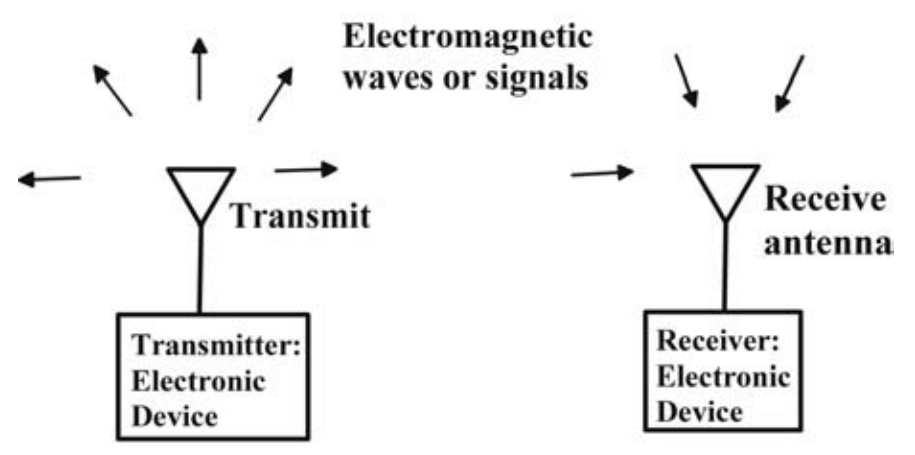
\includegraphics[width=0.6\linewidth]{chapters/figs/fig-2-1}
	\caption{ارسال بی‌سیم از طریق آنتن‌ها.}
	\label{fig:2-1}
\end{figure}




از نظر فیزیکی، یک آنتن آرایشی از رساناها\LTRfootnote{Conductors} و مواد پیرامونی است که در پاسخ به جریان‌ها یا ولتاژهای اعمال‌شده به آن، امواج الکترومغناطیسی تابشی\LTRfootnote{Radiating} تولید می‌کند و یا در اثر تابش\LTRfootnote{impinging} امواج الکترومغناطیسی یا سیگنال‌های رادیویی به آن، جریان‌ها و ولتاژهایی در آن القا می‌شود. روش‌های مختلف آرایش یا قرارگیری رساناها و مواد، منجر به ساخت آنتن‌های متنوعی با رفتارها و ویژگی‌های متفاوت می‌شود. شکل \ref{fig:2-2} یک آنتن تک‌قطبی\LTRfootnote{Monopole antenna} نصب‌شده روی یک خودرو برای دریافت پخش رادیویی و یک آنتن میکرواستریپ پچ\LTRfootnote{Microstrip patch antenna} که در برخی تلفن‌های همراه یا \lr{USB}های بی‌سیم دیده می‌شود را نشان می‌دهد.

\begin{figure}[H]
	\centering
	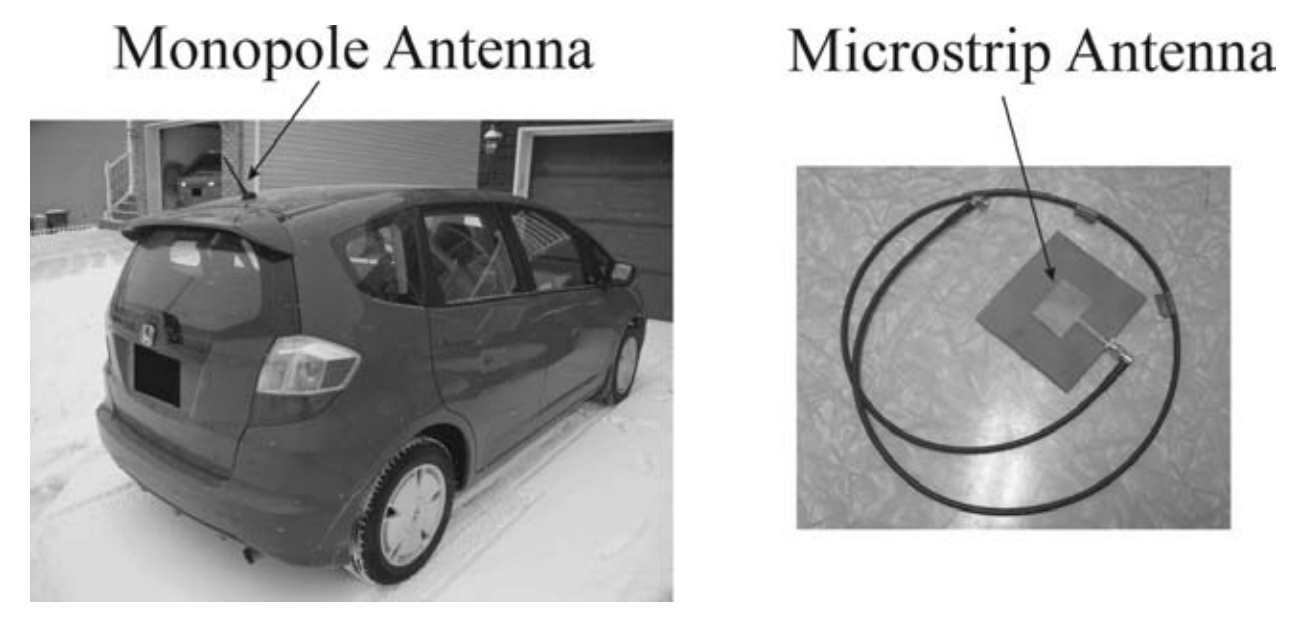
\includegraphics[width=0.7\linewidth]{chapters/figs/fig-2-2}
	\caption{یک آنتن تک‌قطبی نصب‌شده بر روی خودرو و یک آنتن میکرواستریپ پچ.}
	\label{fig:2-2}
\end{figure}

در تئوری، هر دو آنتن فرستنده و گیرنده به دلیل عملکردهای متفاوتشان باید به‌طور جداگانه مطالعه شوند. خوشبختانه، مشخص شده است که توابع فرستندگی و گیرندگی یک آنتن متقابل\LTRfootnote{Reciprocal} هستند. بنابراین، در اکثر متون علمی تاکنون، تنها ویژگی‌های فرستندگی یک آنتن مورد مطالعه و تحلیل قرار گرفته است؛ هنگامی که آنتن برای گیرندگی استفاده می‌شود، ویژگی‌های گیرندگی آن به سادگی و از طریق اصل تقابل\LTRfootnote{Reciprocity} از ویژگی‌های فرستندگی‌اش استخراج می‌شود.

پارامترهای مختلفی برای تعیین کمّی عملکرد یک آنتن معرفی شده‌اند. در این فصل، پارامترها و مفاهیم مهمی را که به تخمین \lr{DOA} مرتبط هستند، شرح خواهیم داد. ابتدا در مورد یک آنتن فرستنده واحد و یک آنتن گیرنده واحد بحث خواهیم کرد و سپس به بررسی آرایه‌های آنتنی\LTRfootnote{Antenna arrays} خواهیم پرداخت که از چندین آنتن واحد تشکیل شده و برای تخمین \lr{DOA} به کار می‌روند.




\section{آنتن فرستنده واحد}
\label{sec:2-1}

یافته‌ها و اثبات‌های علمی نشان می‌دهند که ویژگی‌های زیر برای یک آنتن فرستنده برقرار است:
\begin{enumerate}
	\item انرژی الکترومغناطیسی تابش‌شده از یک آنتن اغلب به‌طور یکنواخت در فضا توزیع نمی‌شود. شدت تابش معمولاً در یک جهت قوی‌تر از سایر جهت‌ها است.
	\item تمامی فرکانس‌های سیگنال‌های رادیویی به‌طور مؤثر از یک آنتن تابش نمی‌شوند. برخی فرکانس‌ها با بازدهی بسیار بالا به هوا یا محیط منتقل می‌شوند و برخی دیگر اصلاً منتقل نمی‌شوند.
\end{enumerate}

برای توصیف این دو پدیده، پارامترهای زیر برای یک آنتن معرفی شده‌اند:
\begin{enumerate}
	\item جهت‌داری\LTRfootnote{Directivity} و بهره\LTRfootnote{Gain} که میزان تمرکز انرژی در یک جهت توسط آنتن را توصیف می‌کنند؛
	\item الگوی تابش\LTRfootnote{Radiation pattern} که شدت‌های تابش نسبی را در تمامی جهت‌ها نشان می‌دهد؛
	\item مدار رزونانس معادل\LTRfootnote{Equivalent resonant circuit} و پهنای باند\LTRfootnote{Bandwidth} که چگونگی رفتار آنتن را از نظر پاسخ‌های فرکانسی نشان می‌دهند.
\end{enumerate}

\subsection{جهت‌داری و بهره}
\label{subsec:2-1-1}

این دو پارامتر اساساً تعیین می‌کنند که یک آنتن تا چه حد می‌تواند انرژی تابشی خود را در یک جهت خاص متمرکز کند. برای این سنجش کمّی، نیاز به یک آنتن مرجع است. در بیشتر موارد، یک آنتن همه‌جهته\LTRfootnote{Omnidirectional antenna} که به‌طور یکسان در تمام جهت‌ها تابش می‌کند، مطابق شکل \ref{fig:2-3} به‌عنوان آنتن مرجع در نظر گرفته می‌شود.

سپس جهت‌داری یک آنتن به‌صورت نسبت شدت توان تابشی آن در یک جهت به شدت توان آنتن همه‌جهته در همان جهت تعریف می‌شود، در حالی که هر دو آنتن توان کل یکسانی را بتابانند. به عبارت دیگر، جهت‌داری یک آنتن میزان شدت توان آن را نسبت به آنتن مرجع (آنتن ایزوتروپیک\LTRfootnote{Isotropic antenna} همه‌جهته) در یک جهت مشخص و در فاصله‌ای دلخواه اندازه‌گیری می‌کند. اگر جهت‌داری در تمام جهت‌ها برابر با یک باشد، آن آنتن یک آنتن همه‌جهته است.

دقیق‌تر آن است که بگوییم جهت‌داری یک آنتن به جهت‌هایی بستگی دارد که شدت تابش در آن‌ها اندازه‌گیری و با آنتن مرجع مقایسه می‌شود. با این حال، در شرایط عادی، واژه جهت‌داری به \textit{بیشینه جهت‌داری} در میان تمامی جهت‌های یک آنتن اشاره دارد.

بهره یک آنتن مستقیماً با جهت‌داری آن در ارتباط است. بهره برابر است با حاصل‌ضرب جهت‌داری در بازده\LTRfootnote{Efficiency} آنتن. بازده، تلفات اهمی توان داخلی آنتن را در نظر می‌گیرد و برابر است با نسبت توان کل تابش‌شده به هوا یا یک محیط توسط آنتن به توان ورودی به آنتن از سوی دستگاه الکترونیکی متصل به آن (شکل \ref{fig:2-4} را ببینید). بازده کمتر یا مساوی $100\%$ است. در نتیجه، بهره همواره کمتر یا مساوی جهت‌داری خواهد بود.

\begin{figure}[ht]
	\centering
	%\includegraphics[width=0.7\textwidth]{fig2-3}
	\caption{آنتن همه‌جهته و توزیع تابش آن.}
	\label{fig:2-3}
\end{figure}






\subsection{الگوی تابش}
\label{subsec:2-1-2}

الگوی تابش یک آنتن، الگوی هندسی از شدت‌های نسبی میدانی است که توسط آنتن با توجه به جهت‌های تابش گسیل می‌شود. برای یک آنتن همه‌جهته ایزوتروپیک ایده‌آل، این الگو یک کره خواهد بود؛ به این معنی که شدت تابش تولیدشده در هر جهت یکسان است. با این حال، برای یک دوقطبی\LTRfootnote{Dipole} معمولی، این الگو به شکل یک چنبره\LTRfootnote{Toroid} یا «دونات» خواهد بود. شکل \ref{fig:2-5} الگوهای دو آنتن، یعنی یک دوقطبی و یک شیپوری موج‌بر\LTRfootnote{Waveguide horn} را نشان می‌دهد. در الگوی تابش، شعاع بلندتر الگو نشان‌دهنده شدت تابش قوی‌تر است. با بررسی الگوی تابش یک آنتن، می‌توانیم مشاهده کنیم که آنتن در کدام جهت بیشترین و در کدام جهت کمترین تابش را دارد.

\begin{figure}[ht]
	\centering
	\caption{الگوهای تابش یک دوقطبی و یک شیپوری موج‌بر (موج‌بر با انتهای باز).}
	\label{fig:2-5}
\end{figure}

\subsection{مدارهای رزونانس معادل و پهنای باند}
\label{subsec:2-1-3}

مانند بسیاری از قطعات مبتنی بر میدان، یک آنتن را می‌توان از نظر ولتاژ و جریان ترمینال ورودی، معادل یک مدار رزونانس در نظر گرفت که در شکل \ref{fig:2-6} نشان داده شده است. در این مدار، علاوه بر مقاومتی که نشان‌دهنده تلفات توان اهمی داخلی آنتن است، مقاومت دیگری به نام مقاومت تابشی\LTRfootnote{Radiation resistor} وجود دارد که میزان توان تابش‌شده به هوا یا محیط را توصیف می‌کند. سلف و خازن نشان‌دهنده ماهیت گزینش‌گر فرکانس\LTRfootnote{Frequency-selective} آنتن هستند. سیگنال‌های ورودی با فرکانس‌های نزدیک به فرکانس رزونانس آنتن می‌توانند به‌راحتی وارد مقاومت تابشی شده و به‌طور معادل، انرژی خود را به هوا یا محیط ارسال کنند.

رابطه معمول بین توان ورودی و فرکانس در شکل \ref{fig:2-7} نشان داده شده است. همانند تعریف پهنای باند برای یک مدار رزونانس، تفاضل بین دو نقطه فرکانسی که در آن‌ها توان به نیمی از مقدار بیشینه خود کاهش می‌یابد، به‌عنوان پهنای باند آنتن تعریف می‌شود. در محدوده پهنای باند، میزان تابش توان را قابل‌قبول در نظر می‌گیریم.

\begin{figure}[ht]
	\centering
	\caption{آنتن و مدار معادل آن.}
	\label{fig:2-6}
\end{figure}

\section{آنتن گیرنده واحد}
\label{sec:2-2}

همان‌طور که پیش‌تر ذکر شد، یک آنتن گیرنده عکس عمل آنتن فرستنده را انجام می‌دهد: انرژی الکترومغناطیسی را در هوا یا محیط جذب و شکار کرده و آن را به جریان‌ها و ولتاژها تبدیل می‌کند. از نظر تئوری، یک آنتن گیرنده نیز باید پارامترهای مخصوص به خود را برای تعیین کمّی عملکردش داشته باشد. به‌ویژه، باید دارای جهت‌داری، بهره و الگوی دریافت مختص به خود باشد که توصیف می‌کنند چگونه یک آنتن گیرنده مقادیر مختلف انرژی سیگنال‌های الکترومغناطیسی یا رادیویی را که از جهت‌های مختلف می‌آیند، در مقایسه با یک آنتن گیرنده همه‌جهته جذب می‌کند. با این حال، مشخص شده است و می‌توان اثبات کرد که این پارامترها دارای مقادیر یا شکلی مشابه با جهت‌داری، بهره و الگوی فرستندگی هستند، مشروط بر اینکه از همان آنتن برای ارسال استفاده شود. در نتیجه، در تقریباً تمامی تحلیل‌های آنتن، جهت‌داری، بهره و الگوی تابش به مواردی ارجاع داده می‌شوند که آنتن برای ارسال استفاده می‌شود. به عبارت دیگر، هنگامی که قرار است از یک آنتن برای دریافت استفاده شود، پارامترهای گیرندگی آن به سادگی از پارامترهای فرستندگی در زمان تحلیل آنتن در حالت ارسال گرفته می‌شوند؛ با این حال، مدار معادل یک استثنا است.

مدار معادل یک آنتن گیرنده در شکل \ref{fig:2-8} نشان داده شده است. این مدار دقیقاً مشابه مدار معادل آنتن در حالت ارسال است، با این تفاوت که یک منبع ولتاژ یا جریان به آن اضافه شده است. منبع جریان نشان‌دهنده جریان معادل القا شده ناشی از حضور میدان‌های الکترومغناطیسی در نزدیکی آنتن گیرنده است. مقاومت‌ها، سلف و خازن مشابه پارامترهای آنتن فرستنده باقی می‌مانند.

\begin{figure}[ht]
	\centering
	\caption{یک رابطه معمول بین فرکانس و توان ورودی به آنتن.}
	\label{fig:2-7}
\end{figure}

\begin{figure}[ht]
	\centering
	%\includegraphics[width=0.7\textwidth]{fig2-8}
	\caption{مدار معادل یک آنتن گیرنده.}
	\label{fig:2-8}
\end{figure}






\section{آرایه آنتنی}
\label{sec:2-3}

آرایه آنتنی\LTRfootnote{Antenna array} گروهی از آنتن‌ها است که برای ارسال یا دریافت سیگنال‌های یکسان استفاده می‌شوند. هر آنتن مجزا اغلب یک عنصر آرایه\LTRfootnote{Array element} نامیده می‌شود. برای یک آرایه گیرنده، سیگنال‌های دریافت شده توسط تمام عناصر آرایه با هم ترکیب شده و سپس برای کاربردهای مختلف، از جمله تخمین \lr{DOA}، پردازش می‌شوند.

به‌منظور تصویرسازی، یک آرایه سه‌عنصری را در نظر بگیرید که به‌طور یکنواخت در امتداد یک خط تراز شده است (شکل \ref{fig:2-9}). راست‌ترین عنصر با شماره $1$ مشخص شده و به‌عنوان عنصر مرجع\LTRfootnote{Reference element} در نظر گرفته می‌شود. دو عنصر دیگر به ترتیب از راست به چپ با شماره‌های $2$ و $3$ نام‌گذاری می‌شوند. فاصله بین دو عنصر مجاور $\Delta$ است. یک منبع امواج الکترومغناطیسی را از چنان فاصله دوری گسیل می‌کند که سه مسیر خطی انتشار از منبع به سه عنصر را می‌توان تقریباً موازی در نظر گرفت. امواج با زاویه $\theta$ به آرایه می‌تابند. در نتیجه، مسیرهای خطی از منبع تا عناصر $2$ و $3$ طولانی‌تر از مسیر تا عنصر $1$ (عنصر مرجع) هستند و این فاصله اضافی برابر است با:
\begin{equation}
	\Delta_m = (m-1) \Delta \sin \theta, \quad m=1, 2, 3
	\label{eq:2-1}
\end{equation}

اکنون فرض کنید سیگنال موج دریافت شده توسط عنصر مرجع (یعنی عنصر $1$)، بدون در نظر گرفتن نویزهای محیط، برابر باشد با:
\begin{equation}
	x_1(t) = s(t)
	\label{eq:2-2}
\end{equation}
در این صورت سیگنال‌های دریافت شده توسط عنصر $2$ و عنصر $3$ را می‌توان به صورت زیر نوشت:
\begin{equation}
	x_2(t) = s(t) e^{-j\beta\Delta_2} = s(t) e^{-j \frac{2\pi}{\lambda} \Delta \sin \theta}
	\label{eq:2-3}
\end{equation}
\begin{equation}
	x_3(t) = s(t) e^{-j\beta\Delta_3} = s(t) e^{-j \frac{2\pi}{\lambda} 2\Delta \sin \theta}
	\label{eq:2-4}
\end{equation}

در اینجا $\beta = 2\pi / \lambda$ ثابت جابجایی فاز\LTRfootnote{Phase shift constant} موج در حال انتشار در هوا و $\lambda$ طول موج است. عبارت جابجایی فاز $e^{-j\beta\Delta_m}$ در روابط \eqref{eq:2-3} و \eqref{eq:2-4}، نتیجه انتشار سیگنال در طول مسیر اضافی $\Delta_m$ در مقایسه با مسیرِ رسیدن به راست‌ترین عنصر است \cite{1}.

در یک حالت کلی‌تر، سیگنال‌های دریافت شده توسط این سه عنصر را می‌توان به صورت زیر نوشت:
\begin{equation}
	\bm{x} = 
	\begin{bmatrix}
		x_1(t) \\
		x_2(t) \\
		x_3(t)
	\end{bmatrix} =
	\begin{bmatrix}
		1 \\
		e^{-j \frac{2\pi}{\lambda} \Delta \sin \theta} \\
		e^{-j \frac{2\pi}{\lambda} 2\Delta \sin \theta}
	\end{bmatrix} s(t) = 
	\begin{bmatrix}
		1 \\
		e^{-j\mu} \\
		e^{-j2\mu}
	\end{bmatrix} s(t) = \bm{a}(\mu) s(t)
	\label{eq:2-5}
\end{equation}
که در آن $\mu = \frac{2\pi}{\lambda} \Delta \sin \theta$ و $\bm{a}(\mu) = [1, e^{-j\mu}, e^{-j2\mu}]^T$ است که اغلب بردار هدایت آرایه\LTRfootnote{Array steering vector} نامیده می‌شود.

معادله \eqref{eq:2-5} قابل تعمیم به یک آرایه $M$-عنصری است و می‌توان آن را به صورت زیر بازنویسی کرد:
\begin{equation}
	\bm{x} = 
	\begin{bmatrix}
		x_1(t) \\
		x_2(t) \\
		\vdots \\
		x_M(t)
	\end{bmatrix} = 
	\begin{bmatrix}
		1 \\
		e^{-j \frac{2\pi}{\lambda} \Delta \sin \theta} \\
		\vdots \\
		e^{-j \frac{2\pi}{\lambda} (M-1)\Delta \sin \theta}
	\end{bmatrix} s(t) = 
	\begin{bmatrix}
		1 \\
		e^{-j\mu} \\
		\vdots \\
		e^{-j(M-1)\mu}
	\end{bmatrix} s(t) = \bm{a}(\mu) s(t)
	\label{eq:2-6}
\end{equation}
و
\begin{equation}
	\bm{a}(\mu) = [1, e^{-j\mu}, \dots, e^{-j(M-1)\mu}]^T
	\nonumber
\end{equation}

اگرچه رابطه \eqref{eq:2-6} برای یک آرایه خطی\LTRfootnote{Linear array} نوشته شده است، اما عبارت $\bm{x} = \bm{a}(\mu)s(t)$ برای هر نوع آرایه دیگری نیز قابل استفاده است.

\begin{figure}[ht]
	\centering
	%\includegraphics[width=0.7\textwidth]{fig2-9}
	\caption{پیکربندی یک آرایه آنتنی سه‌عنصری.}
	\label{fig:2-9}
\end{figure}




\section{نتیجه‌گیری}
\label{sec:2-4}

در این فصل، مفاهیم پایه آنتن‌ها و آرایه‌های آنتنی مرتبط با الگوریتم‌های تخمین \lr{DOA} که در این کتاب مورد بحث قرار می‌گیرند را مرور کردیم. به‌طور خلاصه، آنتن یک دستگاه مبدل است که به منظور ارسال یا دریافت امواج الکترومغناطیسی یا سیگنال‌های رادیویی، میان دستگاه‌های الکترونیکی و هوا (یا یک محیط) واسط می‌شود. این دستگاه می‌تواند ولتاژها/جریان‌ها را به امواج الکترومغناطیسی و بالعکس تبدیل کند. با توجه به این واقعیت که یک آنتن انرژی خود را به‌صورت غیریکنواخت در فضا می‌تاباند، پارامترهایی مانند جهت‌داری، بهره و الگوی تابش اغلب برای تعیین کمّی عملکرد یک آنتن استفاده می‌شوند. از آنجا که آنتن گزینش‌گر فرکانس نیز هست، می‌توان یک مدار معادل را برای توصیف آنتن بر حسب ولتاژ و جریان ترمینال معرفی کرد. به دلیل متقابل بودن عملیات ارسال و دریافت یک آنتن، عملکردهای آنتن اغلب بر اساس ویژگی‌های فرستندگی آن بررسی می‌شوند؛ نتایج حاصل را می‌توان مستقیماً برای ارزیابی عملکرد گیرندگی آن به کار برد.

ادبیات گسترده‌ای در زمینه موضوعات مختلف آنتن منتشر شده است. این حجم عظیم از اطلاعات موجود معمولاً متخصصان حوزه‌های غیرآنتنی را در انتخاب یک متن مناسب به‌عنوان نقطه شروع دچار سردرگمی می‌کند. برای جلوگیری از سردرگمی مشابه، در این فصل تنها به یک مرجع بسنده می‌کنیم. این مرجع، کتاب درسی عالی نوشته‌ی \lr{C. A. Balanis} \cite{1} است؛ این کتاب مقدمه‌ای بر موضوعات مختلف فناوری‌های آنتن، شامل مفاهیم پایه آنتن‌ها و آرایه‌ها را ارائه می‌دهد؛ محتوای این کتاب برای خوانندگان احتمالی اثر حاضر کاملاً کافی است.










	% !TeX root = ../DoABook.tex

\chapter{نمای کلی الگوریتم‌های پایه تخمین \lr{DOA}}
\label{chap:3}

\section{مقدمه}
\label{sec:3-1}

این فصل نمایی کلی از برخی الگوریتم‌های محبوب برای تخمین \lr{DOA} را ارائه می‌دهد. به‌طور کلی، تکنیک‌های تخمین جهت ورود (\lr{DOA}) را می‌توان به‌طور گسترده به سه دسته تکنیک‌های شکل‌دهی پرتو متعارف\LTRfootnote{Conventional beamforming techniques}، تکنیک‌های مبتنی بر زیرفضا\LTRfootnote{Subspace-based techniques} و تکنیک‌های بیشینه درست‌نمایی\LTRfootnote{Maximum likelihood techniques} تقسیم‌بندی کرد.

ساختار این فصل به شرح زیر است: در بخش \ref{sec:3-1}، مدل سیگنال و داده مورد استفاده در این کتاب توصیف می‌شود. برای تشریح این مدل، از یک آرایه خطی یکنواخت استفاده شده است. در بخش \ref{sec:3-2}، مفهوم آرایه‌های حسگری مرکز-متقارن\LTRfootnote{Centro-symmetric sensor arrays} که مورد نیاز بسیاری از الگوریتم‌های \lr{DOA} هستند، مورد بحث قرار می‌گیرد. دو نوع از این آرایه‌ها، یعنی آرایه خطی یکنواخت (\lr{ULA})\LTRfootnote{Uniform Linear Array (ULA)} و آرایه مستطیلی یکنواخت (\lr{URA})\LTRfootnote{Uniform Rectangular Array (URA)}، توصیف می‌شوند. در ادامه، اصول اولیه چند الگوریتم پایه متعلق به هر یک از دسته‌های \lr{DOA} به‌طور خلاصه مورد بحث قرار می‌گیرند.

یک رساله دکتری عالی در زمینه پردازش سیگنال آرایه‌ای برای تخمین‌های \lr{DOA} توسط \lr{M. Haardt} در انتشارات \textit{شاکر ورلاگ} منتشر شده است \cite{1}. این اثر یک بررسی و مطالعه جامع روی یکی از تکنیک‌های \lr{DOA}، یعنی تکنیک \lr{ESPRIT}، ارائه می‌دهد. کتاب حاضر از آن به‌عنوان یکی از مراجع اصلی استفاده می‌کند. به‌منظور تسهیل در بررسی این مرجع اصلی توسط خواننده و جلوگیری از سردرگمی، این کتاب از همان نمادهای ریاضی و اصطلاحات فنی به کار رفته در \cite{1} استفاده می‌کند؛ این نمادها و اصطلاحات در سایر متون علمی مرتبط نیز به کار گرفته شده‌اند.


\section{مدل داده}
\label{sec:3-2}

اکثر رویکردهای مدرن در پردازش سیگنال، مدل‌مبنا\LTRfootnote{Model-based} هستند؛ به این معنی که بر فرضیات خاصی در مورد داده‌های مشاهده‌شده در دنیای واقعی تکیه دارند. مدل داده‌ی غالب که در ادامه این کتاب مورد استفاده قرار می‌گیرد، در این بخش بحث می‌شود.

در سرتاسر توصیف ما از الگوریتم‌های تخمین \lr{DOA}، سناریوی زیر فرض و حفظ شده است \cite{2}:

\begin{itemize}
	\item \textbf{محیط انتشار همسانگرد و خطی\LTRfootnote{Isotropic and linear transmission medium}:} تعداد $d$ منبع وجود دارند که $d$ سیگنال را گسیل می‌کنند؛ این $d$ سیگنال از طریق یک محیط عبور کرده و سپس بر یک آرایه آنتنی یا حسگری $M$-عنصری می‌تابند. فرض می‌شود محیط انتشار بین منابع و آرایه، همسانگرد و خطی است؛ به عبارت دیگر، محیط دارای ویژگی‌های فیزیکی یکسان در تمامی جهت‌های مختلف است و سیگنال‌ها یا امواج در هر نقطه خاص را می‌توان به‌صورت خطی برهم‌نهی کرد. ویژگی همسانگرد و خطی بودن محیط تضمین می‌کند که: (۱) ویژگی انتشار امواج با تغییر \lr{DOA} سیگنال‌ها تغییر نمی‌کند، و (۲) سیگنال‌هایی که در محیط حرکت کرده و سپس توسط هر عنصر از آرایه $M$-عنصری دریافت می‌شوند، می‌توانند به‌عنوان برهم‌نهی خطی $d$ جبهه موج سیگنالِ تولیدشده توسط $d$ منبع محاسبه شوند. علاوه بر این، بهره هر آنتن یا عنصر حسگر برابر با یک فرض می‌شود.
	
	\item \textbf{فرض میدان‌دور\LTRfootnote{Far-field assumption}:} منابع سیگنال $d$ در فاصله‌ای دور از آرایه قرار دارند، به‌طوری که جبهه موج تولیدشده توسط هر منبع با جهت انتشار یکسان به تمامی عناصر می‌رسد و جبهه موج تخت است (تقریب میدان‌دور). بنابراین، میدان‌های در حال انتشار $d$ سیگنال که به آرایه رسیده‌اند، نسبت به یکدیگر موازی در نظر گرفته می‌شوند. این فرض به‌طور کلی با بزرگتر در نظر گرفتن فاصله بین منابع سیگنال و آرایه نسبت به ابعاد آرایه آنتن محقق می‌شود. یک قاعده سرانگشتی این است که فاصله بزرگتر از $2D^2/\lambda$ باشد که در آن $D$ ابعاد آرایه و $\lambda$ طول موج سیگنال‌ها است \cite{3}.
	
	\item \textbf{فرض باندباریک\LTRfootnote{Narrowband assumption}:} سیگنال‌های $d$ از منابع $d$ دارای فرکانس حامل یکسانی هستند، به‌طوری که محتوای فرکانسی آن‌ها در مجاورت فرکانس حامل $f_c$ متمرکز شده است. در این صورت، از نظر ریاضی، هر یک از سیگنال‌های لحظه‌ای که از منابع خارج می‌شوند را می‌توان به‌صورت زیر بیان کرد:
	\begin{equation}
		s_i^r(t) = \alpha_i(t) \cos[2\pi f_c t + \beta_i(t)], \quad 1 \leq i \leq d
		\label{eq:3-1}
	\end{equation}
	سیگنال‌ها تا زمانی باندباریک محسوب می‌شوند که دامنه $\alpha_i(t)$ و فاز حامل اطلاعات $\beta_i(t)$ آن‌ها نسبت به $\tau$ (زمان انتشار سیگنال‌های موج از یک عنصر به عنصر دیگر) به‌کندی تغییر کنند. به عبارت دیگر:
	\begin{equation}
		\alpha_i(t - \tau) \approx \alpha_i(t) \quad \text{و} \quad \beta_i(t - \tau) \approx \beta_i(t)
		\label{eq:3-2}
	\end{equation}
	تغییرات کند $\alpha_i(t)$ و فازهای $\beta_i(t)$ تضمین می‌کنند که تبدیل فوریه رابطه \eqref{eq:3-1} بیشترین محتوای فرکانسی را در همسایگی فرکانس حامل $f_c$ داشته باشد. با تعریف پوش مختلط\LTRfootnote{Complex envelope} سیگنال یا فازور\LTRfootnote{Phasor} به‌صورت زیر، می‌توان به عبارتی مناسب برای تحلیل‌های ریاضی دست یافت:
	\begin{equation}
		s_i(t) = s_{env, i}(t) = \alpha_i(t) e^{j\beta_i(t)} \quad \text{به‌طوری که} \quad s_i^r(t) = \text{Re}\{s_i(t) e^{j 2\pi f_c t}\}
		\label{eq:3-3}
	\end{equation}
	این شکل از سیگنال‌های مختلط (یا تحلیلی) توسط اکثر گیرنده‌ها پشتیبانی می‌شود که سیگنال‌های دریافتی را به هر دو مؤلفه هم‌فاز (بخش حقیقی) و مؤلفه متعامد (بخش موهومی) تجزیه می‌کنند.
	
	\item \textbf{کانال \lr{AWGN}\LTRfootnote{Additive White Gaussian Noise (AWGN)}:} فرض می‌شود نویز یک فرآیند گاوسی سفید مختلط است. نویز جمع‌شونده از یک فرآیند تصادفی با میانگین صفر و از نظر مکانی ناهمبسته\LTRfootnote{Spatially uncorrelated} در نظر گرفته می‌شود که با سیگنال‌ها نیز ناهمبسته است. نویزها در تمامی عناصر آرایه دارای واریانس مشترک $\sigma_N^2$ بوده و بین تمامی عناصر یا حسگرها ناهمبسته هستند.
\end{itemize}

شکل \ref{fig:3-1} سناریوی مربوط به فرضیات فوق را ترسیم می‌کند.


\begin{figure}[ht]
	\centering
	\caption{سناریوی مورد بررسی در این کتاب.}
	\label{fig:3-1}
\end{figure}

\subsection{آرایه خطی یکنواخت (\lr{ULA})}
\label{subsec:3-2-1}

اکنون یک آرایه خطی یکنواخت\LTRfootnote{Uniform Linear Array (ULA)} شامل $M$ عنصر یکسان و همه‌جهته را در نظر بگیرید که روی یک خط تراز شده و دارای فواصل یکسان هستند. فرض کنید فاصله بین دو عنصر مجاور $\Delta$ و فاصله بین منبع و اولین عنصر (راست‌ترین عنصر) $d_d$ باشد. این پیکربندی در شکل \ref{fig:3-2} نشان داده شده است.

فرض کنید یک سیگنال موج تخت تولیدشده توسط منبع $i$ با زاویه $\theta_i$ بر آرایه می‌تابد. سیگنال تولیدشده توسط منبع $i$ یک سیگنال باندباریک $s_i^r(t)$ است که مسافت $d_d$ را با سرعت $c$ طی کرده \cite{3} و به اولین عنصر (راست‌ترین عنصر) می‌رسد. به عبارت دیگر، سیگنال دریافت شده توسط راست‌ترین عنصر، نسخه تأخیریافته‌ی $s_i^r(t)$ با تأخیر $\tau_d = d_d/c$ است. یعنی:
\begin{equation}
	s_{i1}^r(t) = s_i^r(t-\tau_d) = \alpha_i(t-\tau_d) \cos[2\pi f_c(t-\tau_d) + \beta_i(t-\tau_d)] = \text{Re}\{s_{i1}(t) e^{j2\pi f_c t}\}
	\label{eq:3-4}
\end{equation}
که در آن سیگنال فازور متناظر به‌صورت $s_{i1}(t) = \alpha_i(t-\tau_d) e^{j[-2\pi f_c \tau_d + \beta_i(t-\tau_d)]}$ است.

از آنجا که در \lr{ULA} عناصر آرایه روی یک خط قرار دارند، سیگنالی که به عنصر $m$-ام می‌رسد، مسافت بیشتری را نسبت به سیگنال رسیده به راست‌ترین عنصر طی خواهد کرد (شکل \ref{fig:3-2} را ببینید). این مسافت اضافی به‌صورت زیر محاسبه می‌شود:
\begin{equation}
	\Delta_{mi} = (m-1) \Delta \sin \theta_i, \quad m=1, 2, \dots, M
	\label{eq:3-5}
\end{equation}
بنابراین، سیگنالی که به عنصر $m$-ام می‌رسد، دچار تأخیر اضافی می‌شود که برابر است با:
\begin{equation}
	\tau_{mi} = \frac{\Delta_{mi}}{c} = \frac{(m-1) \Delta \sin \theta_i}{c}
	\label{eq:3-6}
\end{equation}

سیگنال دریافت شده توسط عنصر $m$-ام، نسخه تأخیریافته‌ی سیگنال $s_{i1}^r(t)$ (که توسط عنصر اول دریافت شده) با تأخیر اضافی $\tau_{mi}$ است:
\begin{align}
	s_{im}^r(t) &= s_{i1}^r(t-\tau_{mi}) = s_i^r(t-\tau_d-\tau_{mi}) \nonumber \\
	&= \alpha_i(t-\tau_d-\tau_{mi}) \cos[2\pi f_c(t-\tau_d-\tau_{mi}) + \beta_i(t-\tau_d-\tau_{mi})] \nonumber \\
	&\approx \alpha_i(t-\tau_d) \cos[2\pi f_c(t-\tau_d) + \beta_i(t-\tau_d) - (m-1)\mu_i] \nonumber \\
	&= \text{Re}\{s_{i1}(t) e^{j2\pi f_c t} e^{-j(m-1)\mu_i}\}
	\label{eq:3-7}
\end{align}
که در آن $\mu_i = \frac{2\pi f_c \Delta}{c} \sin \theta_i = \frac{2\pi \Delta}{\lambda} \sin \theta_i$ است؛ این مقدار فرکانس مکانی\LTRfootnote{Spatial frequency} نامیده می‌شود که به منبع $i$-ام با زاویه تابش $\theta_i$ اختصاص دارد. $\lambda = c/f_c$ نشان‌دهنده طول موج متناظر با فرکانس حامل $f_c$ است. در استخراج رابطه \eqref{eq:3-7}، تقریب \eqref{eq:3-2} اعمال شده است.

در قالب فازور مختلط، سیگنال دریافتی فوق متناظر است با:
\begin{equation}
	s_{im}(t) \approx \alpha_i(t-\tau_d) e^{j[-2\pi f_c \tau_d + \beta_i(t-\tau_d)]} e^{-j(m-1)\mu_i} = s_{i1}(t) e^{-j(m-1)\mu_i}
	\label{eq:3-8}
\end{equation}

رابطه \eqref{eq:3-8} نشان می‌دهد سیگنالی که توسط عنصر $m$-ام از منبع $i$-ام دریافت می‌شود، مشابه سیگنال دریافت شده توسط عنصر اول (راست‌ترین عنصر) است، اما یک فاکتور جابجایی فاز اضافی به‌صورت $e^{-j(m-1)\mu_i}$ دارد؛ این فاکتور تنها به فرکانس مکانی $\mu_i$ و موقعیت عنصر نسبت به عنصر اول بستگی دارد. برای هر زاویه تابش $\theta_i$ که یک منبع را مشخص می‌کند، یک فرکانس مکانی متناظر $\mu_i$ وجود دارد. بنابراین، هدف کلی از تخمین \lr{DOA} (یعنی $\theta_i$) استخراج این فرکانس مکانی $\mu_i$ از سیگنال‌های دریافت شده توسط آرایه است.

به‌منظور تعیین یکتای $\theta_i$ از روی $\mu_i$، وجود یک تناظر یک‌به‌یک بین آن‌ها الزامی است. در نتیجه، فرکانس‌های مکانی $\mu_i$ به بازه $[-\pi, \pi]$ محدود شده و محدوده \lr{DOA}های ممکن به بازه $[-90^\circ, 90^\circ]$ محدود می‌گردد. این امر به نوبه خود مستلزم آن است که فاصله بین عناصر در شرط $\Delta \leq \lambda/2$ صدق کند. اگر فاصله عناصر در این رابطه صدق نکند، در تعیین \lr{DOA} ابهام به وجود می‌آید، یعنی برای یک مقدار مشخص $\mu_i$، دو راه حل برای زوایا وجود خواهد داشت؛ این وضعیت منجر به ایجاد لوب‌های گریتینگ\LTRfootnote{Grating lobes} در آرایه می‌شود: لوب‌هایی غیر از لوب اصلی که اجازه ورود سیگنال‌ها را از جهت‌های نامطلوب می‌دهند. از نظر فنی، این پدیده علی‌اسینگ مکانی\LTRfootnote{Spatial aliasing} نامیده می‌شود. این مفهوم مشابه نرخ نمونه‌برداری نایکوئیست در تحلیل حوزه فرکانس یک سیگنال است.



\begin{figure}[ht]
	\centering
	\caption{مدل داده برای تخمین \lr{DOA} مربوط به $d$ منبع با یک آرایه خطی $M$-عنصری.}
	\label{fig:3-2}
\end{figure}

اکنون با در نظر گرفتن تمامی سیگنال‌های تولیدشده توسط هر $d$ منبع، $s_i(t)$ برای $1 \le i \le d$، سیگنال کل و نویزهای دریافت شده توسط عنصر $m$-ام در زمان $t$ را می‌توان به‌صورت زیر بیان کرد:
\begin{equation}
	x_m(t) = \sum_{i=1}^{d} s_{im}(t) + n_m(t) = \sum_{i=1}^{d} s_i(t) e^{-j(m-1)\mu_i} + n_m(t), \quad m = 1, 2, \dots, M
	\label{eq:3-9}
\end{equation}


برای تفکیک سیگنال‌های خالص تولیدشده توسط منابع و سیگنال‌های دریافتی یا آشکارسازی‌شده‌ی آلوده به نویز، از این پس به مورد دوم «داده»\LTRfootnote{Data} اطلاق شده و با نماد $\bm{x}$ نشان داده می‌شود.

رابطه \eqref{eq:3-9} را می‌توان به فرم ماتریسی زیر نوشت:
\begin{equation}
	\bm{x}(t) = [\bm{a}(\mu_1), \bm{a}(\mu_2), \dots, \bm{a}(\mu_d)] \bm{s}(t) + \bm{n}(t) = \bm{A}\bm{s}(t) + \bm{n}(t)
	\label{eq:3-10}
\end{equation}
که در آن $\bm{x}(t) = [x_1(t), x_2(t), \dots, x_M(t)]^T$ بردار ستونی داده‌های دریافتی توسط آرایه، $\bm{s}(t) = [s_1(t), s_2(t), \dots, s_d(t)]^T$ بردار ستونی سیگنال‌های تولیدشده توسط منابع و $\bm{n}(t) = [n_1(t), n_2(t), \dots, n_M(t)]^T$ نویزهای جمع‌شونده با میانگین صفر و از نظر مکانی ناهمبسته با ماتریس کوواریانس مکانی برابر با $\sigma_N^2 \bm{I}_M$ است. بردار ستونی هدایت آرایه $\bm{a}(\mu_i)$ به‌صورت زیر تعریف می‌شود:
\begin{equation}
	\bm{a}(\mu_i) = [1, e^{-j\mu_i}, e^{-j2\mu_i}, \dots, e^{-j(M-1)\mu_i}]^T
	\label{eq:3-11}
\end{equation}
این بردار تابعی از فرکانس‌های مکانی ناشناخته $\mu_i$ است و ستون‌های ماتریس هدایت $\bm{A}$ با ابعاد $M \times d$ را تشکیل می‌دهد:
\begin{equation}
	\bm{A} = [\bm{a}(\mu_1), \bm{a}(\mu_2), \dots, \bm{a}(\mu_d)] = 
	\begin{bmatrix} 
		1 & 1 & \dots & 1 \\
		e^{-j\mu_1} & e^{-j\mu_2} & \dots & e^{-j\mu_d} \\
		\vdots & \vdots & \ddots & \vdots \\
		e^{-j(M-1)\mu_1} & e^{-j(M-1)\mu_2} & \dots & e^{-j(M-1)\mu_d}
	\end{bmatrix}
	\label{eq:3-12}
\end{equation}

بسته به پیکربندی‌های مختلف یک آرایه، ماتریس‌های هدایت آرایه‌ای متفاوتی می‌تواند تشکیل شود. بسیاری از الگوریتم‌ها به‌طور خاص مستلزم آن هستند که آرایه‌ها دارای پیکربندی‌های مرکز-متقارن باشند [4]. خوشبختانه، بسیاری از پیکربندی‌های مورد استفاده، مانند آرایه خطی یکنواخت و آرایه مستطیلی، این شرط را برآورده می‌کنند. در بخش بعدی، دو آرایه مرکز-متقارن بسیار رایج را مرور می‌کنیم: \lr{ULA} و \lr{URA}.





\section{آرایه‌های حسگری مرکز-متقارن}
\label{sec:3-3}

در این بخش، تعاریف اولیه آرایه‌های مرکز-هرمیتی\LTRfootnote{Centro-Hermitian} و مرکز-متقارن\LTRfootnote{Centro-symmetric} ارائه می‌شود. این آرایه‌ها به‌دلیل دارا بودن ویژگی‌های خاص، اغلب در کاربردهای عملی مورد استفاده قرار می‌گیرند و معمولاً توسط ماتریس‌های مرکز-متقارن و مرکز-هرمیتی توصیف می‌شوند. در این بخش، بر اساس توصیفات ارائه شده در \cite{1, 5}، به تشریح آن‌ها خواهیم پرداخت.

ابتدا، اجازه دهید $\mathbb{C}^{p \times q}$ را به‌عنوان مجموعه یا فضای ماتریس‌های $p \times q$ در نظر بگیریم. تعاریف زیر بیانگر ماهیت یک ماتریس مرکز-متقارن یا مرکز-هرمیتی است.

\textbf{تعریف ۳-۱} \\
یک ماتریس مختلط $\bm{M} \in \mathbb{C}^{p \times q}$ مرکز-متقارن نامیده می‌شود \cite{1, 5} اگر:
\begin{equation}
	\bm{\Pi}_p \bm{M} \bm{\Pi}_q = \bm{M}
	\label{eq:3-13}
\end{equation}
در اینجا $\bm{\Pi}_p$ ماتریس تعویض\LTRfootnote{Exchange matrix} $p \times p$ است که در پیوست A.2 تعریف شده است؛ این ماتریس روی قطر فرعی (\textit{antidiagonal}) خود دارای مقدار یک و در سایر جاها دارای مقدار صفر است:
\begin{equation}
	\bm{\Pi}_p = 
	\begin{bmatrix}
		0 & \dots & 0 & 1 \\
		0 & \dots & 1 & 0 \\
		\vdots & \dots & \vdots & \vdots \\
		1 & \dots & 0 & 0
	\end{bmatrix}
	\label{eq:3-14}
\end{equation}
اثبات این مطلب دشوار نیست که پیش‌ضرب یک ماتریس در $\bm{\Pi}_p$، ترتیب سطرهای آن ماتریس را معکوس می‌کند (یعنی سطر اول به سطر آخر، سطر دوم به سطر یکی مانده به آخر و سطر آخر به سطر اول تبدیل می‌شود و به همین ترتیب). پس‌ضرب یک ماتریس در $\bm{\Pi}_p$ نیز ترتیب ستون‌های آن را معکوس می‌نماید (یعنی ستون اول به ستون آخر، ستون دوم به ستون یکی مانده به آخر و ستون آخر به ستون اول تبدیل می‌شود). به همین ترتیب، $\bm{\Pi}_q$ ماتریس تعویض $q \times q$ است.

شرط \eqref{eq:3-13} اساساً بیان می‌کند که $\bm{M} \in \mathbb{C}^{p \times q}$ دارای یک مرکز وارونگی\LTRfootnote{Inversion center} است: زمانی که $\bm{M}$ به اندازه ۱۸۰ درجه چرخانده شود، با ماتریس اصلی یکسان خواهد بود. از نظر مکانی، این بدان معناست که به ازای هر نقطه $(x, y, z)$، یک نقطه متمایزناپذیر\LTRfootnote{Indistinguishable} $(-x, -y, -z)$ وجود دارد.

یک ماتریس مختلط $\bm{M} \in \mathbb{C}^{p \times q}$ را مرکز-هرمیتی-متقارن\LTRfootnote{Centro-Hermitian-symmetric} می‌نامند اگر \cite{1, 5}:
\begin{equation}
	\bm{\Pi}_p \bar{\bm{M}} \bm{\Pi}_q = \bm{M}
	\label{eq:3-15}
\end{equation}
که در آن $\bar{\bm{M}}$ مزدوج مختلط $\bm{M}$ است.

شرط \eqref{eq:3-15} در اصل بیان می‌کند که $\bm{M} \in \mathbb{C}^{p \times q}$ دارای یک مرکز وارونگی مزدوج است؛ بدین معنا که وقتی $\bm{M}$ مزدوج شده و سپس ۱۸۰ درجه چرخانده شود، با ماتریس اصلی یکسان می‌گردد. از نظر مکانی، می‌توان دید که به ازای هر نقطه $(x, y, z)$، یک نقطه مزدوج متمایزناپذیر $(-x, -y, -z)$ وجود دارد.

\textbf{تعریف ۳-۲} \\
ماتریس $\bm{Q} \in \mathbb{C}^{p \times q}$ که در رابطه زیر صدق کند:
\begin{equation}
	\bm{\Pi}_p \bar{\bm{Q}} = \bm{Q} \iff \bar{\bm{Q}} = \bm{\Pi}_p \bm{Q}
	\label{eq:3-16}
\end{equation}
ماتریس متقارن حقیقی-چپ-$\bm{\Pi}$\LTRfootnote{Left $\Pi$ real symmetric matrix} نامیده می‌شود.

برای مثال، ماتریس‌های یکانی\LTRfootnote{Unitary matrices}:
\begin{equation}
	\bm{Q}_{2n} = \frac{1}{\sqrt{2}} 
	\begin{bmatrix}
		\bm{I}_n & j\bm{I}_n \\
		\bm{\Pi}_n & -j\bm{\Pi}_n
	\end{bmatrix}
	, \quad 
	\bm{Q}_{2n+1} = \frac{1}{\sqrt{2}} 
	\begin{bmatrix}
		\bm{I}_n & \bm{0} & j\bm{I}_n \\
		\bm{0}^T & \sqrt{2} & \bm{0}^T \\
		\bm{\Pi}_n & \bm{0} & -j\bm{\Pi}_n
	\end{bmatrix}
	\label{eq:3-17}
\end{equation}
به‌ترتیب ماتریس‌های حقیقی-چپ-$\bm{\Pi}$ از مرتبه‌های زوج و فرد هستند. در اینجا $\bm{I}_n$ ماتریس واحد با ابعاد $n \times n$ است. ماتریس‌های حقیقی-چپ-$\bm{\Pi}$ را می‌توان با پس‌ضرب یک ماتریس حقیقی-چپ-$\bm{\Pi}$ مانند $\bm{Q} \in \mathbb{C}^{p \times q}$ در یک ماتریس حقیقی دلخواه $\bm{R}$ نیز به‌دست آورد. یعنی برای هر ماتریس حقیقی-چپ-$\bm{\Pi}$ مانند $\bm{Q}$:
\begin{equation}
	\bm{Q}_r = \bm{QR}, \quad \bm{R} \in \mathbb{R}^{q \times r}
	\label{eq:3-18}
\end{equation}
نیز یک ماتریس حقیقی-چپ-$\bm{\Pi}$ خواهد بود.




\begin{definition}
	یک آرایه حسگری شامل $M$ عنصر، آرایه‌ای مرکز-متقارن\LTRfootnote{Centro-symmetric array} محسوب می‌شود، مشروط بر آنکه مکان عناصر آن نسبت به مرکز هندسی\LTRfootnote{Centroid} متقارن بوده و ویژگی‌های تابشی\LTRfootnote{Radiation characteristics} عناصر جفت‌شده یکسان باشد. بنابراین، می‌توان اثبات کرد که ماتریس هدایت آرایه آن‌ها، $\bm{A}$، در رابطه زیر صدق می‌کند:
	\begin{equation}
		\bm{\Pi}_M \bar{\bm{A}} = \bm{A} \bm{\Lambda}
		\label{eq:3-19}
	\end{equation}
	که در آن $\bm{\Lambda}$ یک ماتریس قطری یکانی\LTRfootnote{Unitary diagonal matrix} است. توجه داشته باشید که در اینجا فرض شده است عناصر حسگر دارای ویژگی‌های تابشی یکسانی هستند.
\end{definition}

در بخش بعدی، دو آرایه مرکز-متقارن پرکاربرد، یعنی آرایه خطی یکنواخت (\lr{ULA}) و آرایه مستطیلی یکنواخت (\lr{URA})، مورد بحث قرار گرفته و روابط مربوط به داده‌ها و ماتریس هدایت آرایه آن‌ها استخراج خواهد شد.



\subsection{آرایه خطی یکنواخت}
\label{subsec:3-3-1}

اکنون مورد آرایه خطی یکنواخت (\lr{ULA}) را در نظر بگیرید که از جمله رایج‌ترین آرایه‌های مورد استفاده در عمل است. یک نمونه پیکربندی در شکل \ref{fig:3-2} نشان داده شده است. همان‌طور که در بخش \ref{sec:3-2-1} توصیف شد، بردار هدایت آرایه متناظر با فرکانس مکانی $\mu_i = - \frac{2\pi}{\lambda} \Delta \sin \theta_i$ را می‌توان به‌صورت زیر نوشت:
\begin{equation}
	\bm{a}(\mu_i) = [1, e^{-j\mu_i}, e^{-j2\mu_i}, \dots, e^{-j(M-1)\mu_i}]^T, \quad 1 \leq i \leq d
	\label{eq:3-20}
\end{equation}
و ماتریس هدایت $\bm{A}$ دارای ساختار وندرموند\LTRfootnote{Vandermonde structure} زیر است:
\begin{equation}
	\bm{A} = [\bm{a}(\mu_1), \bm{a}(\mu_2), \dots, \bm{a}(\mu_d)] = 
	\begin{bmatrix} 
		1 & 1 & \dots & 1 \\
		e^{-j\mu_1} & e^{-j\mu_2} & \dots & e^{-j\mu_d} \\
		\vdots & \vdots & \ddots & \vdots \\
		e^{-j(M-1)\mu_1} & e^{-j(M-1)\mu_2} & \dots & e^{-j(M-1)\mu_d}
	\end{bmatrix}
	\label{eq:3-21}
\end{equation}
آرایه‌های \lr{ULA} مرکز-متقارن هستند، زیرا رابطه زیر به‌سادگی قابل اثبات است:
\begin{equation}
	\bm{\Pi}_M \bar{\bm{A}} = \bm{A} \bm{\Lambda}_\mu
	\label{eq:3-22}
\end{equation}
که در آن
\begin{equation}
	\bm{\Lambda}_\mu = 
	\begin{bmatrix} 
		e^{j(M-1)\mu_1} & 0 & \dots & 0 \\
		0 & e^{j(M-1)\mu_2} & \dots & 0 \\
		\vdots & \vdots & \ddots & \vdots \\
		0 & 0 & \dots & e^{j(M-1)\mu_d}
	\end{bmatrix}
	\nonumber
\end{equation}


بار دیگر، اگر مرکز آرایه به‌عنوان مرجع فاز\LTRfootnote{Phase reference} انتخاب شود، ماتریس هدایت آرایه حاصل، $\bm{A}_c$، را می‌توان با مقیاس‌دهی ستون‌های $\bm{A}$ به صورت زیر به‌دست آورد:
\begin{equation}
	\bm{A}_c = \bm{A} \cdot \bm{\Phi}^{-\frac{M-1}{2}}
	\label{eq:3-23}
\end{equation}
نشان دادن این موضوع دشوار نیست که $\bm{A}_c$ در رابطه \eqref{eq:3-13} صدق می‌کند؛ بنابراین $\bm{A}_c$ مرکز-متقارن است. این نتیجه در فصل \ref{chap:5} مورد استفاده قرار خواهد گرفت. بردارهای هدایت این آرایه، یعنی ستون‌های $\bm{A}_c$ عبارت‌اند از:
\begin{equation}
	\bm{a}_M(\mu_i) = e^{j\frac{M-1}{2}\mu_i} [1, e^{-j\mu_i}, e^{-j2\mu_i}, \dots, e^{-j(M-1)\mu_i}]^T, \quad 1 \leq i \leq d
	\label{eq:3-24}
\end{equation}
در اینجا، زیرنویس $M$ نشان‌دهنده بعد بردار هدایت حقیقی-چپ-$\bm{\Pi}$ یعنی $\bm{a}_M(\mu_i)$ است.

\subsection{آرایه مستطیلی یکنواخت (\lr{URA})}
\label{subsec:3-3-2}
زمانی که هدف، تخمین زوایای یک منبع در هر دو حالت سمت\LTRfootnote{Azimuth} و ارتفاع\LTRfootnote{Elevation} باشد، مطابق شکل \ref{fig:3-3} از آرایه‌های دوبعدی استفاده می‌شود. نمونه‌ای از پیکربندی چنین آرایه‌ای در شکل \ref{fig:3-4} نشان داده شده است. این شکل شامل سه فرم مختلف از جای‌گذاری عناصر آرایه است؛ برخی بدون عناصر مرکزی [شکل \ref{fig:3-4}(b)]، در حالی که برخی دیگر شامل خطوط متعامد از عناصر آرایه‌ای با مراکز فاز مشترک هستند [شکل \ref{fig:3-4}(a, c)] \cite{6}.

\begin{figure}[ht]
	\centering
	%\includegraphics[width=0.7\textwidth]{fig3-3}
	\caption{تعریف زوایای سمت و ارتفاع.}
	\label{fig:3-3}
\end{figure}

\begin{figure}[ht]
	\centering
	%\includegraphics[width=0.8\textwidth]{fig3-4}
	\caption{پیکربندی‌های آرایه دوبعدی مرکز-متقارن (الف-ج).}
	\label{fig:3-4}
\end{figure}


حال شکل \ref{fig:3-4}(الف) را در نظر می‌گیریم. ابعاد آرایه دوبعدی $M_x \times M_y$ است. عناصر آرایه با $(k_x, k_y)$ شماره‌گذاری می‌شوند که در آن $1 \leq k_x \leq M_x$ و $1 \leq k_y \leq M_y$ است. با پیروی از مدل داده‌ای که پیش‌تر توصیف شد، فرض می‌کنیم $d$ سیگنال باندباریک با طول موج $\lambda$ توسط $d$ منبع گسیل می‌شوند و جبهه موج تختِ سیگنال از منبع $i$-ام با زاویه سمت $\phi_i$ و زاویه ارتفاع $\theta_i$ بر آرایه می‌تابد ($1 \leq i \leq d$) (شکل \ref{fig:3-3} را ببینید). فرض کنید:
\begin{equation}
	u_i = \cos \phi_i \sin \theta_i, \quad v_i = \sin \phi_i \sin \theta_i, \quad 1 \leq i \leq d
	\label{eq:3-25}
\end{equation}
قرار می‌دهیم:
\begin{equation}
	\xi_i = \sin \theta_i e^{j \phi_i} = u_i + jv_i
	\label{eq:3-26}
\end{equation}
فرمول ساده‌ای برای تعیین زاویه سمت $\phi_i$ و ارتفاع $\theta_i$ به‌ترتیب از روی کسینوس‌های هادی\LTRfootnote{Direction cosines} متناظر $u_i$ و $v_i$ به‌صورت زیر ارائه می‌شود:
\begin{equation}
	\phi_i = \arg(\xi_i) \quad \text{و} \quad \theta_i = \arcsin(|\xi_i|)
	\label{eq:3-27}
\end{equation}
معادله \eqref{eq:3-27} نشان می‌دهد که تعیین \lr{DOA} یک منبع، معادل با تعیین کسینوس‌های هادی متناظر $u_i$ و $v_i$ است.

اگر داده‌های دریافت شده توسط عنصر آرایه $(k_x, k_y)$ در اسنپ‌شات\LTRfootnote{Snapshot} زمانی $t = t_n$ به‌صورت $x(t_n, k_x, k_y)$ داده شود، در هر اسنپ‌شات $M = M_x \cdot M_y$ نمونه وجود خواهد داشت. با تعمیم نتیجه یک‌بعدی \eqref{eq:3-9}، یافتن برهم‌نهی $d$ سیگنال و نویزهای دریافت شده توسط این عنصر دشوار نیست که به‌صورت زیر نوشته می‌شود:













	
\end{document}